\section{Velvet FlyClient}
\label{sec:flyclient}
We now describe an explicit attack against
the FlyClient protocol under velvet fork deployment.
This is a variation of our Chainsewing Attack of Section~\ref{sec:attack}.
%\subsection{The FlyClient Protocol}
%	The FlyClient protocol suggests that block headers additionaly include an MMR root of all the blocks in the chain. The protocol uses this root hash in multiple ways, both for chain synchronization and specific block queries. Consider a block $b$ which is appended to the chain $\chain$ at height $h_b$:
%	\begin{itemize}
%		\item the prover generates a merkle inclusion proof $\Pi_b$ for the existence of $b$ at height $h_b$ in $\chain$ with respect to the MMR root included in the \emph{tip} of the stable chain $\chain[-1]$
%		\item the verifier receives the merkle root of the chain and an inclusion proof $\Pi_b$ for block $b$ from a prover. He also generates, from $\Pi_b$, the root of the MMR subtree of all blocks in $\chain$ from genesis up to $\chain[h_b - 1]$ and verifies that it is equal to the merkle root included in the header of block $b$.
%	\end{itemize}
%	The above proofs are produced with respect to the MMR root included in $\chain[-1]$.
%
%	\vspace{2mm}
%	\noindent
%	A high level description of the FlyClient is as follows. Consider a verifier, a superlight client, that asks to synchronize to the current longest valid chain. Suppose that he receives different proofs from two provers. Each prover sends (the header) of the last block in the chain, $\chain[-1]$, and a claim for the number of blocks in his chain, $\lvert \chain \rvert$ (which he will later be interrogated upon). If both proofs are valid, then the one claiming the greater block count is selected. The validity check of a proof goes as follows.
%	The verifier has received $\chain[-1]$, $\lvert \chain \rvert$ and queries $k$ random block headers from each prover based on a specific probabilistic sampling algorithm. For each queried block $B_i$ the prover sends the header of $B_i$ along with an MMR subtree inclusion proof $\Pi_{B_i}$ that $B_i$ is the $i_\text{th}$ block in the chain. The verifier also checks that $B_i$ is normally mined on the same chain as $\chain[-1]$ by verifying that the root included in $B_i$ is the MMR root of the first ($\lvert \chain \rvert - 1$) blocks' subtree. If the $k$ random sampled blocks successfully pass through this verification procedure then the proof is considered valid, otherwise the proof is rejected by the verifier.
%	The chain synchronization protocol is given in Algorithm~\ref{alg:flyclient_suffix_protocol}.
%
%	\begin{algorithm}[h]
%		\caption{\label{alg:flyclient_suffix_protocol}FlyClient suffix protocol~\cite{flyclient}}
%		\begin{flushleft}
%		A verifier performs the following steps speaking with two provers who want to convince him that they hold a valid chain of length $n+1$. At least one of the provers is honest. If the provers claim different lengths for their claims then the longer chain is checked first.
%		\begin{enumerate}
%			\item The provers send to the verifier the last block header in their chain. Each header includes the root of an MMR created over the first $n$ blocks of the corresponding chain.
%			\item The verifier queries $k$ random block headers from each prover based on a probabilistic sampling algorithm~\cite{flyclient}.
%			\item For each queried block, $B_i$, the prover sends the header of $B_i$ along with an MMR proof $\Pi_{B_i \in \chain}$ that $B_i$ is the $i-$th block in the chain,
%					  and that $B$'s MMR contents form a prefix of the MMR included in $\chain$.
%			\item The client performs the above checks for each block $B_i$ according to the previous step.
%			\item The client rejects the proof if any checks fail.
%			\item Otherwise, the client accepts $\chain$ as the valid chain.
%		\end{enumerate}
%		\end{flushleft}
%	\end{algorithm}
%
%	\begin{algorithm}[h!]
%		\caption{\label{alg:flyclient_iinfix_protocol}FlyClient infix protocol~\cite{flyclient}}
%		\begin{flushleft}
%		The verifier queries the prover for the header and MMR proof for a single block $b$ in the prover's chain of $n+1$ blocks.
%		\begin{center}
%			\textbf{Verifier}
%		\end{center}
%		\begin{enumerate}
%			\item Has the root of the MMR of $n$ blocks stored in the header of $C[-1]$
%			\item Queries prover for the header of block $b$ and for $\Pi_{b \in C}$
%			\item Checks the validity of the MMR inclusion proof $\Pi_{b \in C}$
%			\item Checks that the MMR of $b$ has contents that are a prefix of the MMR of $C[-1]$
%			\item If everything checks out, accepts the block proof
%		\end{enumerate}
%		\begin{center}
%			\textbf{Prover}
%		\end{center}
%		\begin{enumerate}
%			\item Has chain of $n+1$ blocks and the MMR of the first $n$ blocks
%			\item Receives query for block $b$ from verifier
%			\item Calculates $\Pi_{b \in C}$ from MMR$_C$
%			\item Sends header of $b$ and $\Pi_{b \in C}$ to verifier
%		\end{enumerate}
%		\end{flushleft}
%	\end{algorithm}
%
%	Once the longest chain has been chosen, the infix validation is similar to the previous algorithm.
%	The verifier is synchronized to a chain $\chain$ and already has the tip of the chain $\chain[-1]$. He then queries the prover and receives the header of the specific block of interest $B$ in $\chain$ and the inclusion proof $\Pi_{B \in \chain}$. Then the verifier checks the validity of $B$ in the same way as already described for the random sampled blocks in the synchronization protocol.
%	The prover/verifier single-query protocol is given in Algorithm~\ref{alg:flyclient_iinfix_protocol}.
%\subsection{Velvet MMRs}
	For the FlyClient protocol upgraded miners additionally include an MMR root in each block's header.
    The claim made in the paper is that an honest prover could produce proofs
    by utilizing only the upgraded blocks and that the velvet proofs remain secure even if only a small fraction of miners upgrade. 
    %The velvet protocol is susceptible to a chainsewing attack, succeeding with non-negligible probability.
    %We now give a high-level overview of this attack.
	%As already described so far, velvet fork requires any block to be accepted in the chain regardless of the validity of the auxiliary data coming with the protocol update.
    Due to the velvet conditions, an adversary may append blocks in $\chain$ that contain invalid MMR information.
    As an example, consider an invalid MMR that omits blocks existing in $\chain$ or contains blocks which belong in temporary forks of $\chain$.
    We will use the same terminology as in velvet superblocks and refer to a block that contains an invalid MMR as \emph{thorny}, while to one with valid MMR as \emph{smooth}.
    Any upgraded block can be thorny or smooth.

%\subsection{The Attack}
	Consider the security impact of thorny blocks in the FlyClient protocol.
	Due to the velvet FlyClient description being only partial, we
	make a couple of assumptions considering how thorny blocks are treated by the velvet version of the protocol.
	First, when constructing a new block's MMR, the honest miner should treat thorny blocks as unupgraded, 
	i.e., ignore invalid MMRs and build on top of the MMR of the most recent smooth block. 
	%For this observe that when creating a new block, an upgraded \emph{miner} must include an MMR
	%commiting to all previous blocks (upgraded or not, thorny or not). 
	This rule is of great importance and, to our opinion, inevitable, since if miners do not verify the 
	validity of previous blocks' MMRs, the adversary could trivially attack the protocol by mining a thorny block in $\chain$ and have all subsequent upgraded
	blocks commit to an invalid chain history.  
	%%%  In essence, a thorny block in $\chain$ could suggest an invalid chain and it is vital that, whereas such a block will be accepted in $\chain$, honest upgraded miners continue to 
	%%% produce valid MMR commitments in subsequent blocks.
	
	A FlyClient proof contains the chain tip $C[-1]$, which must be an upgraded block because of its vital importance in the protocol with respect to MMR consistency checks of the sampled blocks. 
	Upon receiving a proof the verifier interrogates the prover. During the interrogation, each sampled block $b$ may
	be upgraded or not. In case $b$ does not contain an MMR (i.e., $b$ is an unupgraded block), the verifier cannot check MMR consistency
	between $b$ and $C[-1]$, so the verifier checks MMR validity between $C[-1]$ and the closest upgraded descendant of $b$.
	Since both smooth and thorny blocks may exist in $\chain$ this MMR validity check could fail, as one of the blocks may be smooth while the other one thorny.
	In this case the verifier will search for the next closest upgraded descendant of $b$ and repeat the procedure until a consistent descendant is found or reject 
	the proof\footnote{
	In reality it is prover's responsibility to construct a proof so that the verifier can immediately select the first valid upgraded descendant. We continue 
	with this description as it is equivalent and more intuitive.
	}.
	Because of the velvet conditions, the verifier must accept that some consistency checks between $b$ and $C[-1]$ will fail.
	On the other hand, and this denotes the second assumption, the verifier cannot allow any number of inconsinstencies freely. To see why,
	consider the following attack. Let the honest chain have three consecutive blocks $b_i$, $b_{i+1}, b_{i+2}$ at heights $i, i+1, i+2$ respectively. The attacker 
	produces a thorny block $b'_{i+1}$ on top of $b_i$ containing a double spend transaction in conflict with $b_{i+1}$.
	Whenever she wants to convince the verifier that the honest chain contains $b'_{i+1}$ she produces another thorny block $b_j$ on top of the current chain's tip 
	and sends her proof. Note that $b_j$ is a thorny block that contains an MMR that includes
	$b'_{i+1}$. The adversary claims that $b'_{i+1}$ and $b_j$ are the only smooth blocks in the chain, contrary to reality, where all \emph{other} upgraded blocks 
	are non-thorny.
	More specifically $b_j$ will appear in the proof as it is the tip of the chain, while $b_{i+1}$ will be in the proof
	only if it is selected by the random sampler. Her proof will only be found invalid if the random sampler queries both blocks at heights $i+1, i+2$, so that 
	the invalid prevId pointer shows up. The attacker can decrease this probability
	by letting the chain grow enough before attempting to construct a proof, as the random sampler chooses older blocks with lower probability 
	(the probability of this sampling occuring is negligible if the proof size is logarithmic). 
	When the verifier receives two valid proofs of the same length, one from the attacker and one from an honest node,
	the verifier cannot tell which proof is the correct one. 
	One mechanism to avoid this attack is to have the verifier count how many of
	the MMR verifications are successful. In the case of the above attack, most upgraded blocks will appear inconsistent with the claimed (thorny) tip.
	Intuitively, under an appropriate velvet honest majority assumption, and for sufficiently long underlying chains, the honest proof (ending in a smooth block)
	will pass more consistency checks among the samples performed
	by the verifier, as compared to the adversarial proof (ending in a thorny block).
	We conclude that an appropriately designed velvet variant of the FlyClient protocol must compare proofs depending on how many
	consistency checks pass or, put in another way, compare the upgraded hashing power included in the proofs. 

	Now, considering this favourable version of the FlyClient protocol, we give a sketch of a more sophisticated attack which works
	even when the adversary is bounded to $1/2$ of the upgraded mining power.
    The adversary acts as follows.
		She initially creates a transaction in an honest block $b$. She subsequently forks from the parent of $b$ to create a block $b'$ containing
		a double spend.
    Afterwards she mines block $a'$ in the honest chain, $\chain_B$, which includes an MMR root containing $b'$ instead of $b$.
    Next she keeps mining blocks on top of the honest chain, ensuring that they contain MMR commitments to
		$a'$, $b'$ and the whole other honest chain, excluding $b$.
    Additionally, during this period when she mines on $\chain_B$ she tries to suppress any honest upgraded block in $\chain_B$ by mining selfishly.
    When an honest upgraded block $\chain[i]$ appears she mines on top of block $\chain[i-1]$.
    Even if she mines a block and the suppression fails she can still use her fresh block in her proof by continuing to construct consistent MMRs
    in the coming blocks as described before.
		Figure~\ref{fig:combined_chainsewing_flyclient} illustrates an example of the underlying suppression attack.
    At some point, the adversary produces her proof.
    From the verifier's perspective the black colored blocks form a valid chain,
    since the tip contains consistent MMR commitments with all these blocks.
	
    In conclusion, FlyClient is not secure as-is under velvet conditions. We believe it can be made secure through the construction we propose,
	but further analysis regarding its security assumptions, i.e. a \emph{velvet} honest majority assumption, is required.

	\begin{figure}
		\begin{center}
			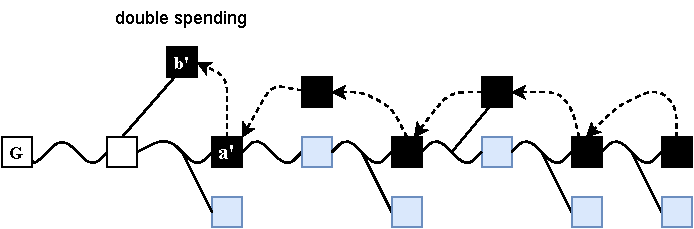
\includegraphics[width=0.95\columnwidth]{figures/flyclient_combined_attack.pdf}
		\end{center}
		\caption{The chainsewing attack. Here, dashed arrows are thorny MMR commitments.}
		\label{fig:combined_chainsewing_flyclient}
	\end{figure}
